\documentclass{article}
\usepackage[utf8] {inputenc}
\renewcommand{\baselinestretch}{1.5}
\title{Livscykelanalys Solceller}
\author{Jonas Cronholm}
\date{May 2021}
\usepackage{graphicx}
\usepackage{hyperref}
\begin{document}
	\pagenumbering{Roman}
	\maketitle
	\pagebreak
	\tableofcontents
	\pagebreak
	
\section{Produktbeskrivning}
%Solpanelerna står för ynkliga 0,2 procent av jordens sammanlagda framställning och utvinning av elektricitet, och 0,2 procent av hela Sveriges elproduktion. Även fast denna siffra må se liten ut på papper så är de den snabbaste växande källa för strömförsörjning och har ökat med hundra procent sedan millennieskiftet.
  
%Solpaneler består av ett ljuskänsligt material som avger elektrisk ström när det bestrålas av en ljuskälla, detta gör solpanelerna mycket lämpliga för elkraftförsörjning inom många områden. Solcellerna är ett försök att fylla det behov som finns för förnybara energikällor för att ersätta de fossila bränslen som nu står för majoriteten av världens elkraftstillverkning. 

%Att utvinna elektrisk ström från ljus är inte en ny upptäckt. Redan år 1839 upptäckte Alexandre-Edmond Bequerel att vissa material avger elektrisk ström när det blir bestrålat av ljus.
%Senare, under 1870-talet så togs ämnet upp igen och forskare som Willoughby Smith och William Grylls Adams påbörjade sin efterforskning. Willoughby kom fram till att ämnet selenium avger elektrisk ström när det bestrålas av ljus.

%Tio år senare lanserades den första kommersiellt tillgängliga solpanelen men den blev mycket ratad och kritiserad på grund av dess mycket låga effektivitet. Det skulle inte vara förrän under mitten av 1900-talet som man började framställa solceller som var baserade på kisel istället för selenium. De flesta solceller som nu används är baserade på kisel eftersom det mer effektivt kan utvinna energi ur ljus. Utvecklingen av solcellerna drivs framåt av tanken om en förnybar, miljövänlig och ekonomiskt hållbar energiutvinningsmetod för att ersätta de mycket skadliga fossila bränslen som står för majoriteten av jordens strömtillförsel. Problemet med global uppvärmning visar att behovet för en sådan produkt är stort och att det börjar bli mycket bråttom att utveckla den. 

%De alternativ som vi redan nu kan se är bland annat vindkraft och vattenkraft, dessa två kräver dock en mellanhand som kan distribuera den producerade elen till kunderna. Man kan inte själv slå upp ett vattenkraftverk på sin tomt, till skillnad från solpaneler som lätt kan installeras hos privatpersoner.
\pagebreak
\newline
%“Livscykelanalys (LCA) används för att bedöma en produkts miljöpåverkan. Solceller och - paneler bedöms baserat på LCA vara bland de mest miljövänliga av alla energi- och elproducerande tekniker (Komoto et al., 2018). I en LCA bedöms ett antal olika miljöpåverkanskategorier och inkluderar livscykelns alla steg; utvinning av råvaror; tillverkning av solceller och solpaneler, import och transporter, installation och montering av 
%solcellssystemet, användningen av panelen och hantering vid bortskaffandet av den (antingen genom återanvändning, återvinning eller slutgiltig kvittblivning)
%” [1]\newline
%Genom denna LCA:n hoppas jag att jag kan framställa en översiktlig bild om hur tillverkningen, transporten, installationen, användningen och återvinningen av solpaneler påverkar dagens miljö, om det är ekologiskt hållbart med solpaneler (bedömt efter mängd av koldioxidutsläpp och effektivitet av solpanelerna) och om det är ekonomiskt hållbart att införskaffa, använda och underhålla solpaneler på en större skala (t.ex. För att driva fabriker etc.). 
\pagebreak
\section{Utvinning av råvaror}
%En typisk kiselsolcellspanel består av en aluminiumram, ett glasskikt, ett inkapslingslager av 
%polyvinyletylacetat, solceller (kisel), en kopplingsbox och en baksida av ett PET eller Tedlar-skikt.

%Jag kommer inte att täcka alla dessa material i denna LCA:n, utan jag kommer att ge en överblick över de två materialen kisel och glas. Detta eftersom kislet är den delen av solpanelerna som reagerar med ljuset för att skapa energi och för att solpaneler innehåller mest glas (efter massa).

%I denna LCA:n tar jag upp EN råvara som utgör grunden för TVÅ material som jag kommer att beskriva och som används i produkten.

%Kisel (Si) är det element som konverterar ljuset till användbar energi. Det är även ett av de materialen som kräver mest energi för att tillverkas. Detta är mestadels på grund av att man behöver använda extrema temperaturer för att omvandla råvaran som man utvinner kislet ur (sand) till en användbar kiseltacka som sedan kan omvandlas till mycket tunna kiselskivor. Man tillsätter även bor för att ge kislet en positiv laddning.
%Glaset används som ett skyddande lager för det dyrbara kiselelementet. Man använder glas istället för andra transparenta material som till exempel plexiglas på grund av dess egenskaper. Bland dessa är att glaset kan beläggas med ett antireflex-lager, (se bild 1).

%Nackdelar med kislet som material är att det är mycket svårt att omvandla från råvara till en användbar produkt och framställningsprocessen är fortfarande mycket dyr. Återanvändning av kisel är också inte helt lätt.
%Nackdelar med glaset som material är att det är mycket känsligt och kan spricka lätt ifall det inte hanteras varsamt. Detta kan leda till många problem inom tillverkningen och att man slösar mycket material.
\pagebreak
%Produktionen av kisel är mycket dyr och energikrävande eftersom den involverar extrema temperaturer. Kislet utvinns från vanlig sand från stranden och förfinas under produktionen. 
%Framställningen av glaset kräver också extrema temperaturer och är därför även ganska energikrävande och man använder ofta naturgas i processen. Glastillverkningen har ett koldioxidutsläpp per ton glas på ungefär 700kg CO2.

\begin{figure}[h]
	\centering
	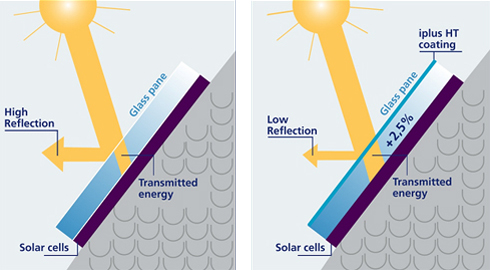
\includegraphics[width=\linewidth]{reflexcoat}
	\caption{Antireflex-lager}
	\label{fig:refl1}
\end{figure}
\pagebreak
\section{Tillverkning och transport}
%Solpaneler tillverkas oftast i Kina, som nästan alla elektroniska apparater. Anledningen till att man oftast väljer att producera sina produkter i Kina är för att det är mycket billigt med arbetskraft. Det beror även på att Kina tillverkar nästan allt man kan tänka sig. Detta leder till att producenter av produkter inte behöver importera varor från andra länder och behöva betala tull och andra avgifter. Den största tillverkaren i världen är LONGi Solar, de har sina fabriker i Shanxiprovinsen. 
%Endast en minoritet av solpanelerna, globalt sätt, tillverkas inom EU.
%Det är bara ett företag (Midsummer AB) i Sverige som idag producerar solpaneler i kommersiell skala. Solpanelerna importeras istället till Sverige av företag som antingen fungerar som grossister för andra solcellsföretag, eller säljer direkt till slutkonsument.

%Produktionen och transportens sammanlagda koldioxidutsläpp kan fördelas på kWh, då hamnar solceller på runt 28-35g CO2/kWh, medans fossila bränslen kan ha utsläpp upp till 1000g CO2/kWh.

%Oftast brukar solcellerna transporteras via färjor och båtar i containrar. Varje container kan hålla mellan tjugo och trettio enheter beroende på beställning. Färjorna transporterar solcellerna till kunden.
\pagebreak
\section{Användning}
%Solceller har en tillämpning inom elindustrin. De finns även i bland annat miniräknare, portabla laddare, klockor och fritidsutrustning som till exempel belysning. När solceller används avger dem inga utsläpp, fast oftast så ackompanjeras en solpanelsgrupp med batterier och en strömkälla som jämnar ut strömbehovet när det inte finns solljus tillgängligt, t.ex. under natten. Sådana strömkällor kan ha koppling till fossila bränslen och kan ha påverkan på miljön. 
%Om man dock räknar in produktionen och transportens sammanlagda koldioxidutsläpp och fördelar det på mängden kWh (kilowattimmar) som solpanelerna producerar så kan man få en ungefärlig siffra på runt 28-35g CO2/kWh, detta är mycket lägre än de olika sorterna fossila bränslen som producerar runt omkring 500-1000g CO2/kWh. (se diagram 1).

\begin{figure}[h]
	\centering
	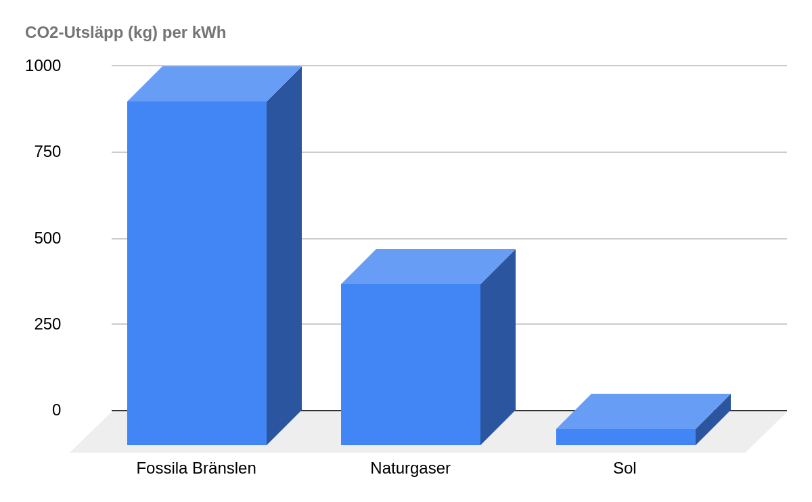
\includegraphics{diagram1}
\caption{Diagram 1.}
\label{fig:dig1}
\end{figure}

%Världens första avfallshanteringsprogram för alla typer av solceller uppnådde år 2016 en återvinningsgrad på 96 procent för kiselbaserade solceller, (enligt \href{https://m.naturskyddsforeningen.se/faqsol}{Svenska Naturskyddsföreningen}
).\newline
%Detta innebär att solpaneler är mycket återvinningsbara.

%För att dessa material skall kunna återanvändas krävs dock återigen energi som man inte kan garantera kommer från förnybara energikällor. 

%Till exempel så används stora mängder glas, som har en smältpunkt på omkring 1500 grader Celsius. Dessa temperaturer uppnås oftast med hjälp av elektroniska ugnar men kan också uppnås med hjälp av oxyfueltekniker som producerar betydligt mindre koldioxidutsläpp.

%Den slutgiltiga återvinningsgraden för de två materialen. (se diagram 2) från “Återvinningsgrader föringående material i kiselbaserade solceller och tunnfilmssolceller" Paiano (2015)

%Kisel 80 procent, Glas 95 procent. 

\begin{figure}[h]
	\centering
	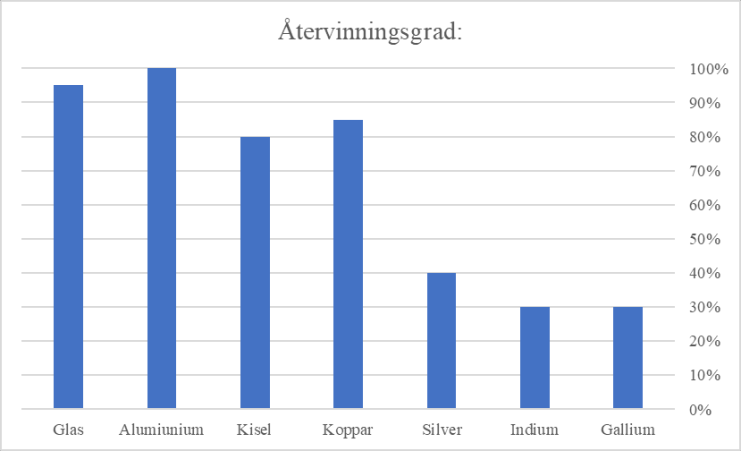
\includegraphics[width=\linewidth]{diagram2}
	\caption{Diagram 2.}
	\label{fig:dig2}
\end{figure}
\pagebreak
\section{Slutsats}

\subsection{Inledning och beskrivning av slutsats}

%I denna livscykelanalys (LCA) har jag diskuterat min produkts påverkan på miljön (bedömt efter mängd av koldioxidutsläpp och effektivitet av solpanelerna) och om det är ekonomiskt hållbart att införskaffa, använda och underhålla solpaneler på en större skala (t.ex. För att driva fabriker etc.). Och även om det lönar sig på en privat skala. Jag ska även diskutera om dagens situation för återvinning är tillräckligt effektiv och hållbar i längden ekologiskt sätt.

\pagebreak

\subsection{Slutsats ur ett hållbarhetsperspektiv}
%Min bedömning av solpanelers ekologiska hållbarhet är att solpaneler är mycket mer hållbara än fossila bränslen och andra skadliga energikällor. De har ett mycket lägre genomsnittligt CO2/kWh-värde än andra elkällor.
%” Under 2016 uppskattades de genomsnittliga utsläppen för solceller variera mellan 20 och 25 g CO2/kWh, baserat på en tillverkning i Kina och något högre solinstrålning än Sveriges. Vid en omräkning för Sveriges solinstrålning varierar utsläppen mellan 28 g och 35 g CO2/kWh. 
%I jämförelse är detta bra mycket lägre än för de fossila energislagen, som genererar ungefär 500 till 1 000 g CO2/kWh.  Det beror på att tillverkningen av solceller är ganska energikrävande och att de idag ofta tillverkas på platser med mycket kolkraft i energimixen, som i Kina och Tyskland. Det finns dock bättre alternativ på marknaden och eftersom större delen av utsläppen är indirekta har solceller potential att få mycket låga utsläpp i framtida energisystem eller vid produktion exempelvis i Sverige. ”
%Slutsats ur ett ekonomiskt perspektiv

%Enligt min bedömning av ekonomisk hållbarhet är att solpanelerna inte kan betala tillbaka den summa som det kostar att investera i en fungerande solpanelsinstallation. Dock är jag optimistisk och tror gärna att det kommer att bli lönsamt inom de kommande 5 åren
%” I dag kostar solceller ungefär 18 000 kr/kW (kronor per kilowatt). En normalstor anläggning för ett hushåll är på 5 kW och kostar då strax under 100 000 kronor. Genom stöd kan investeringskostnaden minska med upp till 20 procent. Solcellerna tar då upp ungefär 30–40 kvadratmeter och under ett år producerar de omkring 5000 kWh (såklart beroende på hur väl solcellen har placerats i förhållande till solen). Det kan jämföras med att boende i en villa använder omkring 5000 kWh hushållsel varje år. Görs både uppvärmning och varmvatten med el kan det kräva ytterligare 20 000 kWh el varje år. Boende i lägenhet använder i snitt omkring 2000 kWh el varje år.”
\pagebreak
\section{Källor}
\href{https://www.naturskyddsforeningen.se/nyheter/solenergin-flodar-men-var-finns-solcellerna}{Naturskyddsföreningen. Okänt datum. Solenergin flödar - men var finns solcellerna?}
(Hämtad 2021-05-16)
\newline
\newline
\href{https://www.greenmatch.co.uk/blog/2014/12/how-are-solar-panels-made}{Greenmatch. 2021. How Are Solar Panels Produced?}
(Hämtad 2021-05-16).
\newline
\newline
\href{https://ec.europa.eu/clima/sites/default/files/ets/allowances/docs/bm_study-glass_en.pdf}{Fraunhofer Institute for Systems and Innovation Research (på uppdrag av EU). 2009. Methodology for the free allocation of emission allowances in the EU ETS post 2012. Sector report for the glass industry.}
(Hämtad 2021-05-16)
\newline
\newline
\href{http://www.viaspace.com/biomass_versus_alternatives.php}{Viaspace. Okänt datum. Biomass Compared to Fossil Fuels, Solar and Wind}
[diagram 1 (data)](Hämtad 2021-05-17)
\newline
\newline
\href{https://www.powerfromsunlight.com/why-solar-panel-glass-is-very-important-when-choosing-solar-panel-type/}{Power from Sunlight. 2017. Why Solar Panel Glass Is Very Important When Choosing Solar Panel Type?}
(Hämtad 2021-05-17)
\newline
\newline
\href{https://lup.lub.lu.se/student-papers/search/publication/9006745}{Ouchterlony, Anna. 2020. Framtida återvinning av solcellspaneler i Sverige. Diss., Lunds Tekniska Högskola.}
(Hämtad 2021-05-16) [1]
\newline
\newline
\href{https://www.google.com/url?sa=i&url=https%3A%2F%2Fpixy.org%2F5941817%2F&psig=AOvVaw0mL8oneRcGAh-b2aowx3Oz&ust=1621416471737000&source=images&cd=vfe&ved=0CA0QjhxqFwoTCJjX35710vACFQAAAAAdAAAAABAD}{Omslagsbild, Petr Kratochvil, solar panels 615x410px.}
Creative Commons Licence version 2.5 CC0
\newline
\newline

(bild 1) http://www.fsolar.de/ (Hämtat från \href{https://www.powerfromsunlight.com/why-solar-panel-glass-is-very-important-when-choosing-solar-panel-type/}{hemsidan}. )
\pagebreak

\subsection{Faktasök och källornas trovärdighet}

\href{https://lup.lub.lu.se/student-papers/search/publication/9006745}{Ouchterlony, Anna. 2020. Framtida återvinning av solcellspaneler i Sverige. Diss., Lunds Tekniska Högskola.}
(Hämtad 2021-05-16)
Denna källa är trovärdig eftersom den är ett högskolearbete på Lunds Tekniska Högskola, den är publicerad på deras hemsida och jag tror att man inte skulle lägga till falsk information i en akademisk uppsats.
\newline
\newline
Naturskyddsföreningen. Okänt datum. Solenergin flödar - men var finns solcellerna?
https://www.naturskyddsforeningen.se/nyheter/solenergin-flodar-men-var-finns-solcellerna
(Hämtad 2021-05-16).
Naturskyddsföreningen är en oberoende organisation som anlitar experter och mycket trovärdiga källor under sin efterforskning. De stärker även sina artiklar med information från forskningar och undersökningar. En nackdel med denna källa är att det sällan står vem som har skrivit själva artikeln.
\newline
\newline
\href{https://www.greenmatch.co.uk/blog/2014/12/how-are-solar-panels-made}{Greenmatch. 2021. How Are Solar Panels Produced?}
(Hämtad 2021-05-16).
Greenmatch är ett brittiskt företag som säljer lösningar inom solenergins värld. Deras artiklar verkar vara väl underbyggda och har stöd från legitim forskning. En nackdel med denna källa är att den är ett företag som säljer tjänster inom det ämnet som analyseras. Detta kan leda till att de glorifierar den verklighet som ligger bakom tillverkningen för att den verkliga informationen skulle leda till en förlust av kunder hos dem.
\newline
\newline
\href{https://ec.europa.eu/clima/sites/default/files/ets/allowances/docs/bm_study-glass_en.pdf}{Fraunhofer Institute for Systems and Innovation Research (på uppdrag av EU). 2009. Methodology for the free allocation of emission allowances in the EU ETS post 2012. Sector report for the glass industry.}
(Hämtad 2021-05-16)
Denna undersökning är på uppdrag av den Europeiska unionen, jag finner det ytterst osannolikt att det skulle tillåtas falsk information i en så pass seriös undersökning. Jag misstänker även att denna text har gått genom flera kontroller innan den publiceras.
\pagebreak

\href{http://www.viaspace.com/biomass_versus_alternatives.php}{Viaspace. Okänt datum. Biomass Compared to Fossil Fuels, Solar and Wind}
[diagram 1 (data)] (Hämtad 2021-05-17)
Viaspace är en privat organisation som fokuserar på förnybara energikällor. Vad gäller deras förtrolighet hittar jag inte särskilt mycket information men deras data i det diagrammet jag skapade verkar vara ganska korrekt med tanke på att ungefär samma data publiceras på andra sidor.
\newline
\newline
\href{https://www.powerfromsunlight.com/why-solar-panel-glass-is-very-important-when-choosing-solar-panel-type/}{Power from Sunlight. 2017. Why Solar Panel Glass Is Very Important When Choosing Solar Panel Type?}
(Hämtad 2021-05-17)
Power from Sunlight är en försäljningssite som säljer produkter och tjänster som involverar solpaneler. Denna källa är nog medelpålitlig eftersom jag nu i efterhand hittar samma information som jag hittade i denna källa på andra ställen. Jag valde denna källa eftersom den förklarade väl hur de olika sorterna av glas och beläggningarna påverkade solpanelens slutgiltiga effektivitet.

\end{document}